% no answer key
% \documentclass[letterpaper]{exam}

% answer key
\documentclass[letterpaper, landscape]{exam}
\usepackage{2in1, lscape} 
\printanswers

\usepackage{units} 
\usepackage{xfrac} 
\usepackage[fleqn]{amsmath}
\usepackage{float}
\usepackage{mdwlist}
\usepackage{booktabs}
\usepackage{cancel}
\usepackage{polynom}
\usepackage{caption}
\usepackage{fullpage}
\usepackage{comment}
\usepackage{enumerate}
\usepackage{graphicx}

\usepackage{mathtools} 

\newcommand{\dg}{\ensuremath{^\circ}} 
\newcommand{\sgn}{\operatorname{sgn}}

\everymath{\displaystyle}
\title{Calculus I \\ Homework Eight \\ Section 2.8}
\author{}
\date{\today}

\begin{document}

  \maketitle

  \ifprintanswers
  \else
  \section{Homework}
    \begin{itemize*}
      \item read Section 2.8
      \item exercises: 1, 3-9, 14, 19-28, 35-37, 41-43
    \end{itemize*}
  \fi

  \ifprintanswers

    \begin{description}

      \item[1] 
        \begin{enumerate}[(a)]
          \item $f'(-3) \approx 1$
          \item $f'(-2) \approx 1$
          \item $f'(-1) \approx 0$
          \item $f'(0) \approx -4$
          \item $f'(1) \approx 0$
          \item $f'(2) \approx 1$
          \item $f'(3) \approx 1$
        \end{enumerate}

      \item[3] 
        \begin{enumerate}[(a)]
          \item \fbox{ II }
          \item \fbox{ IV }
          \item \fbox{ I }
          \item \fbox{ III }
        \end{enumerate}

      \item[4-9] graphs

      \item[14]
        The derivative of $\sin(x)$ looks like $\cos(x)$. See Figure \ref{fig:ex14}.

        \begin{figure}[H]
          \centering
          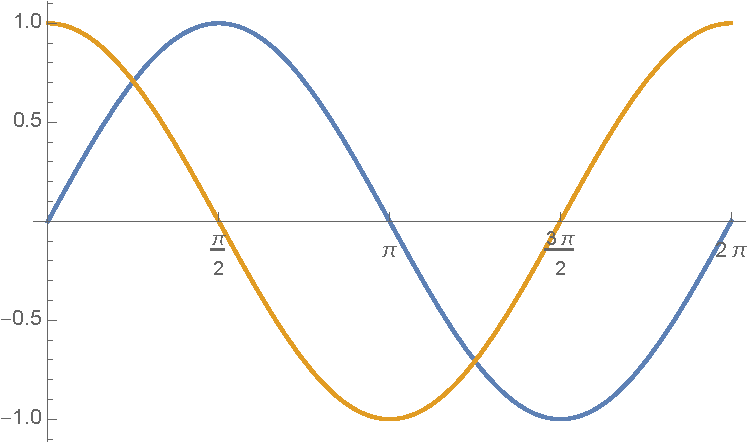
\includegraphics[scale = 0.5]{ex14.pdf}
          \caption{Exercise 15}
          \label{fig:ex14}
        \end{figure}

      \item[19]
        % \begin{tabular}[H]{lll}
        %   \toprule
        %   $f'(x)$ & Domain of $f(x)$ & Domain of $f'(x)$ \\
        %   \midrule
        %   $f'(x) = \frac{1}{2}$ & $f$: $(-\infty, \infty)$ & Domain $f'$: $(-\infty, \infty)$ \\
        %   \bottomrule
        % \end{tabular}

        \[
          f'(x) = \frac{1}{2}
        \]
        \begin{tabular}[H]{lr}
          \toprule
          Domain of $f(x)$  & $(-\infty, \infty)$ \\
          Domain of $f'(x)$ & $(-\infty, \infty)$ \\
          \bottomrule
        \end{tabular}

        % \begin{itemize}
        %   \item $f'(x) = \frac{1}{2}$
        %   \item Domain $f$: $(-\infty, \infty)$
        %   \item Domain $f'$: $(-\infty, \infty)$
        % \end{itemize}

      \item[20]
        \[
          f'(x) = m
        \]
        \begin{tabular}[H]{lr}
          \toprule
          Domain of $f(x)$  & $(-\infty, \infty)$ \\
          Domain of $f'(x)$ & $(-\infty, \infty)$ \\
          \bottomrule
        \end{tabular}

      \item[21]
        \[
          f'(x) = -18t + 5
        \]
        \begin{tabular}[H]{lr}
          \toprule
          Domain of $f(x)$  & $(-\infty, \infty)$ \\
          Domain of $f'(x)$ & $(-\infty, \infty)$ \\
          \bottomrule
        \end{tabular}

      \item[22]
        \[
          f'(x) = 3x - 1
        \]
        \begin{tabular}[H]{lr}
          \toprule
          Domain of $f(x)$  & $(-\infty, \infty)$ \\
          Domain of $f'(x)$ & $(-\infty, \infty)$ \\
          \bottomrule
        \end{tabular}

      \item[23]
        \[
          f'(x) = 3x^2 - 3
        \]
        \begin{tabular}[H]{lr}
          \toprule
          Domain of $f(x)$  & $(-\infty, \infty)$ \\
          Domain of $f'(x)$ & $(-\infty, \infty)$ \\
          \bottomrule
        \end{tabular}

      \item[24]
        \[
          f'(x) = 1 + \frac{1}{ 2 \sqrt{x} }
        \]
        \begin{tabular}[H]{lr}
          \toprule
          Domain of $f(x)$  & $[ 0, \infty )$ \\
          Domain of $f'(x)$ & $( 0, \infty )$ \\
          \bottomrule
        \end{tabular}

      \item[25]
        \[
          f'(x) = \frac{1}{\sqrt{1 + 2x}}
        \]
        \begin{tabular}[H]{lr}
          \toprule
          Domain of $f(x)$  & $\left[ - \frac{1}{2}, \infty \right)$ \\
          Domain of $f'(x)$ & $\left( - \frac{1}{2}, \infty \right)$ \\
          \bottomrule
        \end{tabular}

      \item[26]
        \[
          f'(x) = \frac{10}{(1 - 3x)^2}
        \]
        \begin{tabular}[H]{lr}
          \toprule
          Domain of $f(x)$  & $x \neq \frac{1}{3}$ \\
          Domain of $f'(x)$ & $x \neq \frac{1}{3}$ \\
          \bottomrule
        \end{tabular}

      \item[27]
        \[
          f'(x) = \frac{4}{(t + 1)^2}
        \]
        \begin{tabular}[H]{lr}
          \toprule
          Domain of $f(x)$  & $t \neq -1$ \\
          Domain of $f'(x)$ & $t \neq -1$ \\
          \bottomrule
        \end{tabular}

      \item[28]
        \[
          f'(x) = -\frac{ 1 }{ 2t^{3/2} }
        \]
        \begin{tabular}[H]{lr}
          \toprule
          Domain of $f(x)$  & $(0, \infty)$ \\
          Domain of $f'(x)$ & $(0, \infty)$ \\
          \bottomrule
        \end{tabular}

      \item[35] $x = -4$; $x = 0$

      \item[36] $x = 0$; $x = 3$

      \item[37] $x = -1$; $x = 4$

      \item[41]
        \begin{tabular}[H]{lll}
          \toprule
          Function & Curve & Explanation \\
          \midrule
          $f$      & $a$   & \\
          $f'$     & $b$   & slope of $a$ \\
          $f''$    & $c$   & slope of $b$ \\
          \bottomrule
        \end{tabular}

      \item[42]
        \begin{tabular}[H]{lll}
          \toprule
          Function & Curve & Explanation \\
          \midrule
          $f$      & $d$   & \\
          $f'$     & $c$   & slope of $d$ \\
          $f''$    & $b$   & slope of $c$ \\
          $f'''$   & $a$   & slope of $b$ \\
          \bottomrule
        \end{tabular}

      \item[43]
        \begin{tabular}[H]{lll}
          \toprule
          Function     & Curve & Explanation \\
          \midrule
          position     & $c$   & \\
          velocity     & $b$   & slope of position \\
          acceleration & $a$   & slope of velocity \\
          \bottomrule
        \end{tabular}

     \end{description}
 
  \else
    \vspace{10 cm}
    \begin{quote}
      \begin{em}
        Do you see law and order? There is nothing but disorder, and instead of law there
        is the illusion of security. It is an illusion because it is built on a long
        history of injustices: racism, criminality, and the genocide of millions. Many
        people say it is insane to resist the system, but actually, it is insane not to. 
      \end{em}
    \end{quote}
    \hspace{2 cm} --Mumia Abu-Jamal
  \fi

\end{document}

